\documentclass[preprint, 3p,
authoryear]{elsarticle} %review=doublespace preprint=single 5p=2 column
%%% Begin My package additions %%%%%%%%%%%%%%%%%%%

\usepackage[hyphens]{url}

  \journal{An awesome journal} % Sets Journal name

\usepackage{graphicx}
%%%%%%%%%%%%%%%% end my additions to header

\usepackage[T1]{fontenc}
\usepackage{lmodern}
\usepackage{amssymb,amsmath}
% TODO: Currently lineno needs to be loaded after amsmath because of conflict
% https://github.com/latex-lineno/lineno/issues/5
\usepackage{lineno} % add
\usepackage{ifxetex,ifluatex}
\usepackage{fixltx2e} % provides \textsubscript
% use upquote if available, for straight quotes in verbatim environments
\IfFileExists{upquote.sty}{\usepackage{upquote}}{}
\ifnum 0\ifxetex 1\fi\ifluatex 1\fi=0 % if pdftex
  \usepackage[utf8]{inputenc}
\else % if luatex or xelatex
  \usepackage{fontspec}
  \ifxetex
    \usepackage{xltxtra,xunicode}
  \fi
  \defaultfontfeatures{Mapping=tex-text,Scale=MatchLowercase}
  \newcommand{\euro}{€}
\fi
% use microtype if available
\IfFileExists{microtype.sty}{\usepackage{microtype}}{}
\usepackage[]{natbib}
\bibliographystyle{plainnat}

\ifxetex
  \usepackage[setpagesize=false, % page size defined by xetex
              unicode=false, % unicode breaks when used with xetex
              xetex]{hyperref}
\else
  \usepackage[unicode=true]{hyperref}
\fi
\hypersetup{breaklinks=true,
            bookmarks=true,
            pdfauthor={},
            pdftitle={Short Paper},
            colorlinks=false,
            urlcolor=blue,
            linkcolor=magenta,
            pdfborder={0 0 0}}

\setcounter{secnumdepth}{5}
% Pandoc toggle for numbering sections (defaults to be off)

% Pandoc syntax highlighting
\usepackage{color}
\usepackage{fancyvrb}
\newcommand{\VerbBar}{|}
\newcommand{\VERB}{\Verb[commandchars=\\\{\}]}
\DefineVerbatimEnvironment{Highlighting}{Verbatim}{commandchars=\\\{\}}
% Add ',fontsize=\small' for more characters per line
\usepackage{framed}
\definecolor{shadecolor}{RGB}{248,248,248}
\newenvironment{Shaded}{\begin{snugshade}}{\end{snugshade}}
\newcommand{\AlertTok}[1]{\textcolor[rgb]{0.94,0.16,0.16}{#1}}
\newcommand{\AnnotationTok}[1]{\textcolor[rgb]{0.56,0.35,0.01}{\textbf{\textit{#1}}}}
\newcommand{\AttributeTok}[1]{\textcolor[rgb]{0.13,0.29,0.53}{#1}}
\newcommand{\BaseNTok}[1]{\textcolor[rgb]{0.00,0.00,0.81}{#1}}
\newcommand{\BuiltInTok}[1]{#1}
\newcommand{\CharTok}[1]{\textcolor[rgb]{0.31,0.60,0.02}{#1}}
\newcommand{\CommentTok}[1]{\textcolor[rgb]{0.56,0.35,0.01}{\textit{#1}}}
\newcommand{\CommentVarTok}[1]{\textcolor[rgb]{0.56,0.35,0.01}{\textbf{\textit{#1}}}}
\newcommand{\ConstantTok}[1]{\textcolor[rgb]{0.56,0.35,0.01}{#1}}
\newcommand{\ControlFlowTok}[1]{\textcolor[rgb]{0.13,0.29,0.53}{\textbf{#1}}}
\newcommand{\DataTypeTok}[1]{\textcolor[rgb]{0.13,0.29,0.53}{#1}}
\newcommand{\DecValTok}[1]{\textcolor[rgb]{0.00,0.00,0.81}{#1}}
\newcommand{\DocumentationTok}[1]{\textcolor[rgb]{0.56,0.35,0.01}{\textbf{\textit{#1}}}}
\newcommand{\ErrorTok}[1]{\textcolor[rgb]{0.64,0.00,0.00}{\textbf{#1}}}
\newcommand{\ExtensionTok}[1]{#1}
\newcommand{\FloatTok}[1]{\textcolor[rgb]{0.00,0.00,0.81}{#1}}
\newcommand{\FunctionTok}[1]{\textcolor[rgb]{0.13,0.29,0.53}{\textbf{#1}}}
\newcommand{\ImportTok}[1]{#1}
\newcommand{\InformationTok}[1]{\textcolor[rgb]{0.56,0.35,0.01}{\textbf{\textit{#1}}}}
\newcommand{\KeywordTok}[1]{\textcolor[rgb]{0.13,0.29,0.53}{\textbf{#1}}}
\newcommand{\NormalTok}[1]{#1}
\newcommand{\OperatorTok}[1]{\textcolor[rgb]{0.81,0.36,0.00}{\textbf{#1}}}
\newcommand{\OtherTok}[1]{\textcolor[rgb]{0.56,0.35,0.01}{#1}}
\newcommand{\PreprocessorTok}[1]{\textcolor[rgb]{0.56,0.35,0.01}{\textit{#1}}}
\newcommand{\RegionMarkerTok}[1]{#1}
\newcommand{\SpecialCharTok}[1]{\textcolor[rgb]{0.81,0.36,0.00}{\textbf{#1}}}
\newcommand{\SpecialStringTok}[1]{\textcolor[rgb]{0.31,0.60,0.02}{#1}}
\newcommand{\StringTok}[1]{\textcolor[rgb]{0.31,0.60,0.02}{#1}}
\newcommand{\VariableTok}[1]{\textcolor[rgb]{0.00,0.00,0.00}{#1}}
\newcommand{\VerbatimStringTok}[1]{\textcolor[rgb]{0.31,0.60,0.02}{#1}}
\newcommand{\WarningTok}[1]{\textcolor[rgb]{0.56,0.35,0.01}{\textbf{\textit{#1}}}}

% tightlist command for lists without linebreak
\providecommand{\tightlist}{%
  \setlength{\itemsep}{0pt}\setlength{\parskip}{0pt}}

% From pandoc table feature
\usepackage{longtable,booktabs,array}
\usepackage{calc} % for calculating minipage widths
% Correct order of tables after \paragraph or \subparagraph
\usepackage{etoolbox}
\makeatletter
\patchcmd\longtable{\par}{\if@noskipsec\mbox{}\fi\par}{}{}
\makeatother
% Allow footnotes in longtable head/foot
\IfFileExists{footnotehyper.sty}{\usepackage{footnotehyper}}{\usepackage{footnote}}
\makesavenoteenv{longtable}






\begin{document}


\begin{frontmatter}

  \title{Short Paper}
    \author[Some Institute of Technology]{Irina Vélez%
  \corref{cor1}%
  \fnref{1}}
   \ead{alice@example.com} 
    \author[Another University]{Otto Palkama%
  %
  \fnref{1}}
   \ead{bob@example.com} 
      \affiliation[Some Institute of Technology]{
    organization={Big Wig University},addressline={1 main
street},city={Gotham},postcode={123456},state={State},country={United
States},}
    \affiliation[Another University]{
    organization={Department},addressline={A street
29},city={Manchester,},postcode={2054 NX},country={The Netherlands},}
    \cortext[cor1]{Corresponding author}
    \fntext[1]{This is the first author footnote.}
    \fntext[2]{Another author footnote.}
  
  \begin{abstract}
  This is the abstract.

  It consists of two paragraphs.
  \end{abstract}
    \begin{keyword}
    keyword1 \sep 
    keyword2
  \end{keyword}
  
 \end{frontmatter}

\hypertarget{introduction}{%
\section{1. Introduction}\label{introduction}}

The idea is to explore how the use of Large Language Models (LLMs) as
General Purpose Technology (GPT) could reshape industries, considering
the generalization capabilities of LLMs and the rapid adoption of these
tools by the public and firms.

A. Background on the potential economic impact of Large Language Models
(LLMs) as General Purpose Technology (GPT) B. Objective of the paper:
Exploring how the use of LLMs as GPT could reshape industries and
contribute to economic growth

Generalization of tools seems to be an important characteristic to
leverage the potential of growth and development, because if a same tool
could be broad use for different purposes, so the tool becomes in a very
valuable tool.

Until now the abilities reached by the Large Languages Models LLMs have
arisen to a certain level of computational power that might require
scaling up past this threshold (10\^{}23 training FLOPs), meaning that
they are able to perform multiple tasks related to Text Understanding
and Generation,Problem Solving and Mathematics, Image and Data
Classification, Text Analysis and Comprehension, and so on, but as
\citep{weiemergent} suggested for future works, it could be possible new
abilities could emerge scaling up the models and understanding how
emergence occurs would provide new insights into how to train
more-capable language models.

On the other hand, the use of LLMs as a base technology of other tools,
such as software-AI powered, open a new window and enveloped the
potential of productivity improvements of the work-human force or human
capital as it was mention by \citep{gptaregpts} telling that LLMs such
as GPTs exhibit traits of general-purpose technologies, could have
considerable economic, social, and policy implications.

So, the potential arising of emergent abilities and the wide use of LLMs
as enablers of new tools (AI based-software) alongside the spread use of
tools such as ChatGPT by a large amount of humans (here: million of
users of chatGPT), it could signify a future unseen before by the human
beings, because the expansion and pushing of new boarders and limits
would be accelerated.

\hypertarget{generalization-capabilities-of-llms-as-gpt}{%
\section{Generalization Capabilities of LLMs as
GPT}\label{generalization-capabilities-of-llms-as-gpt}}

A. Examining the adoption rate of previous GPTs B. Key factors
contributing to the widespread adoption of a technology as a GPT C.
Reviewing the literature on the potential of AI as a GPT

Artificial intelligence a term coined by emeritus Stanford Professor
John McCarthy in 1955, was defined by him as ``the science and
engineering of making intelligent machines''.\footnote{Available at:
  https://hai.stanford.edu/sites/default/files/2020-09/AI-Definitions-HAI.pdf}
These systems are designed to simulate human cognitive abilities, such
as learning, reasoning, problem-solving, perception, and language
understanding. Within the realm of AI, Large Language Models (LLMs) are
a specific type of AI model that utilizes deep learning techniques,
particularly neural networks, to process and generate human-like
language. LLMs are trained on vast amounts of text data and can perform
tasks like language translation, text summarization, and question
answering.

In the past, computer programs were developed by painstakingly encoding
human knowledge, following a precise set of instructions that mapped
specific inputs to desired outputs. This approach required programmers
to meticulously define every step of the process. However, machine
learning systems operate differently. They utilize general algorithms,
such as neural networks, which enable them to independently determine
the appropriate mapping between inputs and outputs. This is achieved
through exposure to extensive datasets containing numerous examples. By
analyzing and learning from these examples, machine learning systems can
identify patterns and make accurate predictions or classifications
without explicit programming instructions.

General Purpose Technology is a transformative technology with a strong
improvement process at the begining and eventually becoming widely
adopted for its multiples uses, while producing many spillover effects
\citep{paradox}. As such, it have a pervasive impact on society as a
whole, mainly due to its capability to redefine the ways in which
businesses operate, improve productive and contribute to long-term
economic growth. Some well-know examples are steam power, electricity,
semiconductors, and internet.

\hypertarget{assessing-the-potential-economic-impact}{%
\section{Assessing the Potential Economic
Impact}\label{assessing-the-potential-economic-impact}}

Considering the potential of the AI as a new GPT, specifically the LLMs,
assessing its potential economic impact to setting expectatives, it
could be address based on a retrospective approach what it means that
the behaviour of previous General Purpose Technology like internet,
electricity or semiconductors, can give a more realistic answer to this
question, given the current conditions of uncertainty of this time.

It is worth noting that the article by \citep{paradox} was written seven
years before the launch of ChatGPT by OpenAI. This temporal context adds
significance to the insights provided by \citep{paradox}, as they were
able to anticipate and discuss the potential impact of artificial
intelligence (AI) technologies on productivity growth before the
emergence of specific AI models like ChatGPT. Their analysis and
observations offer valuable perspectives on the productivity paradox and
the clash between expectations and statistical realities in the context
of technologies with the potential to become GPTs.

This apparent incongruence relies on the time lag between invention and
the full impact on the economy and society. It takes time to build the
stock of the new technology, develop the necessary human capital
skillset, undergo the re-engineering process of business process
transformations, and develop complementary innovations for its full
realization.

One example mentioned by \citep{paradox} is the call center industry,
which had approximately 2.2 million agents in the United States. It was
plausible at that time to anticipate that voice recognition systems like
IBM's Watson could potentially reduce the number of workers by 60\%.
However, in hindsight, it is evident that the expectations have not been
fully met, as shown in Figure \ref{fig1}, which illustrates the
statistics.

\begin{figure}

{\centering 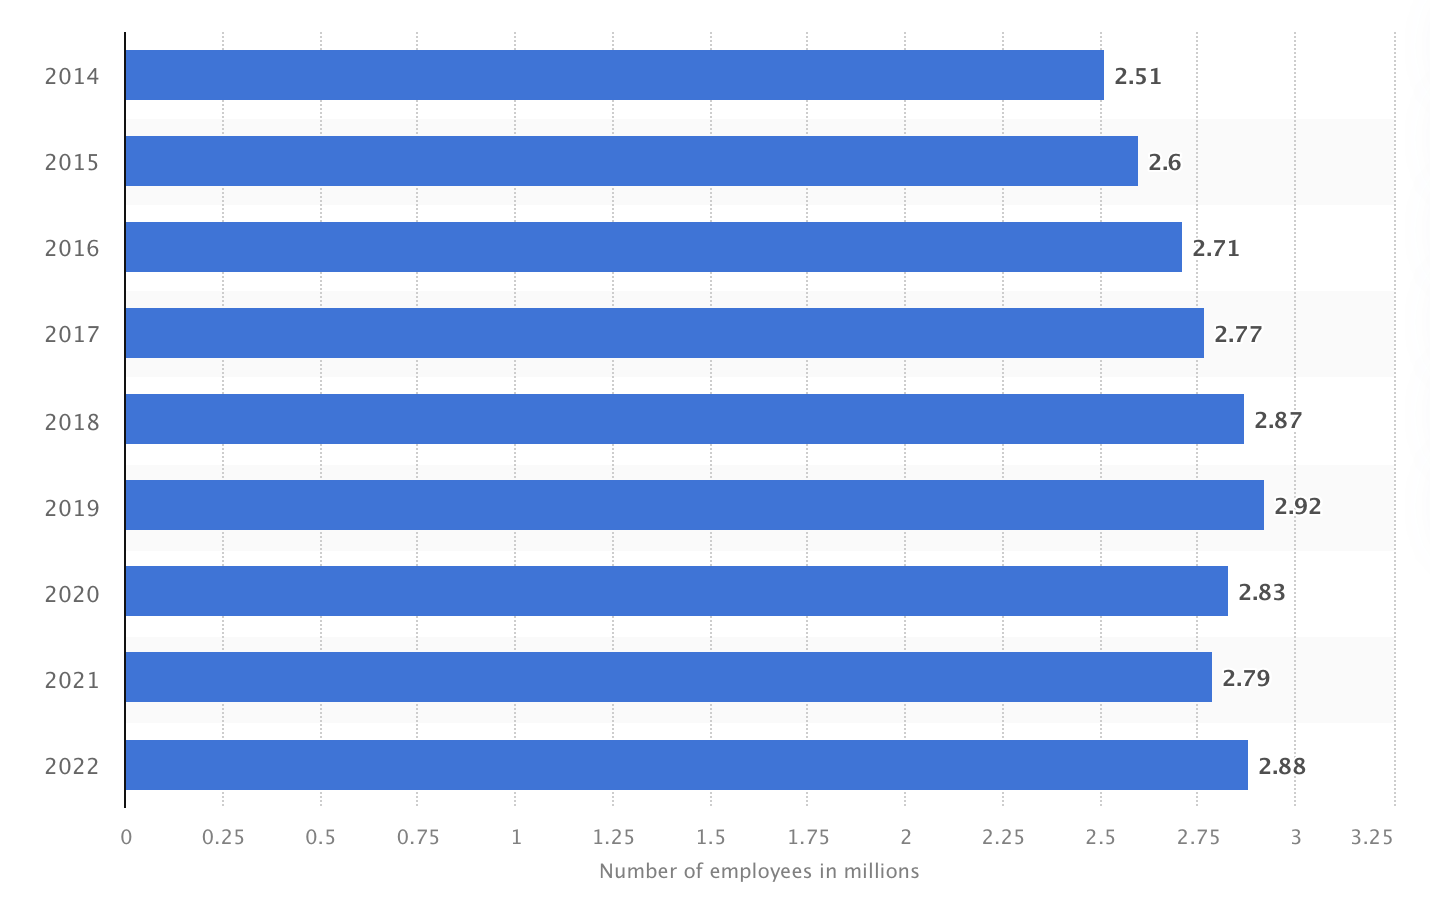
\includegraphics[width=0.7\linewidth]{../Views/contact_center_employees_US} 

}

\caption{\label{fig1}Number on contact center employees in the United States from 2014 to 2022.}\label{fig:fig1}
\end{figure}

The positive expectations surrounding new technologies driving
development, economic growth, and generating profits are often
accompanied by optimism from industry leaders, technology experts, and
venture capitalists. This optimism leads to speculative investments and
forecasts of future company wealth in the financial sector. However, as
\citep{paradox} suggests, there is no inherent contradiction between
forward-looking technological optimism and backward-looking
disappointment. Both can coexist, particularly during periods of
transformative change. This can be attributed to human nature, as
individuals desire to see their expectations fulfilled within their
lifetime. However, it takes time for society to fully incorporate and
benefit from new technologies, resulting in a slower pace of
assimilation.

B. Evaluating the potential economic impact in terms of value creation
and cost optimization 1. Real cases of successful implementations of
LLMs for value creation 2. Real cases of successful implementations of
LLMs for cost optimization

\begin{longtable}[]{@{}
  >{\raggedright\arraybackslash}p{(\columnwidth - 4\tabcolsep) * \real{0.3333}}
  >{\raggedright\arraybackslash}p{(\columnwidth - 4\tabcolsep) * \real{0.3333}}
  >{\raggedright\arraybackslash}p{(\columnwidth - 4\tabcolsep) * \real{0.3333}}@{}}
\toprule\noalign{}
\begin{minipage}[b]{\linewidth}\raggedright
Value Creation
\end{minipage} & \begin{minipage}[b]{\linewidth}\raggedright
Cost Reduction
\end{minipage} & \begin{minipage}[b]{\linewidth}\raggedright
Reference
\end{minipage} \\
\midrule\noalign{}
\endhead
\bottomrule\noalign{}
\endlastfoot
Deep neural network system matches the diagnostic performance of 21
board certified dermatologists in detecting skin cancer. & &
\citep{cancer} \\
Row 2 Value 1 & Row 2 Value 2 & Row 1 Value 2 \\
Row 3 Value 1 & Row 3 Value 2 & Row 1 Value 2 \\
Row 3 Value 1 & Row 3 Value 2 & Row 1 Value 2 \\
\end{longtable}

\begin{center}\rule{0.5\linewidth}{0.5pt}\end{center}

Total Factor Productivity should reflect the exceptional technological
advance

Review data: CBInsights - Labour Productivity Growth vs Global
Investment focused on AI - OECD Productivity Growth - Real Median income
has stagnated since the late 1990s

Both capital deepening and total factor productivity (TFP) growth lead
to labor productivity growth, and both seem to be playing a role in the
slowdown

The old adage that ``past performance is not predictive of future
results'' applies well to trying to predict productivity growth in the
years to come, especially in periods of a decade or longer. Historical
stagnation does not justify forward-looking pessimism. Taken from
Paradox

C. Intangible capital - capital may not be reflected in the measurements
of economic growth

AI developing skills: Perception and cognition

\hypertarget{llms-vs.-artificial-general-intelligence-agi}{%
\section{LLMs vs.~Artificial General Intelligence
(AGI)}\label{llms-vs.-artificial-general-intelligence-agi}}

A. Understanding the difference between LLMs and AGI B. Exploring
whether AGI is the real General Purpose Technology

\hypertarget{acknowledging-benefits-and-limitations-of-llms-as-gpt}{%
\section{Acknowledging Benefits and Limitations of LLMs as
GPT}\label{acknowledging-benefits-and-limitations-of-llms-as-gpt}}

A. Discussing the potential benefits of LLMs as GPT B. Addressing the
limitations and challenges associated with LLMs as GPT

\hypertarget{conclusion}{%
\section{Conclusion}\label{conclusion}}

A. Summarizing the main points discussed in the paper B. Emphasizing the
potential of LLMs as GPT in reshaping industries

\hypertarget{bibliography-styles}{%
\section{Bibliography styles}\label{bibliography-styles}}

Here are two sample references: \citeauthor{Feynman1963118}
\citetext{\citeyear{Feynman1963118}; \citealp{Dirac1953888}}.

By default, natbib will be used with the \texttt{authoryear} style, set
in \texttt{classoption} variable in YAML. You can sets extra options
with \texttt{natbiboptions} variable in YAML header. Example

\begin{Shaded}
\begin{Highlighting}[]
\FunctionTok{natbiboptions}\KeywordTok{:}\AttributeTok{ longnamesfirst,angle,semicolon}
\end{Highlighting}
\end{Shaded}

There are various more specific bibliography styles available at
\url{https://support.stmdocs.in/wiki/index.php?title=Model-wise_bibliographic_style_files}.
To use one of these, add it in the header using, for example,
\texttt{biblio-style:\ model1-num-names}.

\hypertarget{using-csl}{%
\subsection{Using CSL}\label{using-csl}}

If \texttt{citation\_package} is set to \texttt{default} in
\texttt{elsevier\_article()}, then pandoc is used for citations instead
of \texttt{natbib}. In this case, the \texttt{csl} option is used to
format the references. Alternative \texttt{csl} files are available from
\url{https://www.zotero.org/styles?q=elsevier}. These can be downloaded
and stored locally, or the url can be used as in the example header.

\hypertarget{equations}{%
\section{Equations}\label{equations}}

Here is an equation: \[ 
  f_{X}(x) = \left(\frac{\alpha}{\beta}\right)
  \left(\frac{x}{\beta}\right)^{\alpha-1}
  e^{-\left(\frac{x}{\beta}\right)^{\alpha}}; 
  \alpha,\beta,x > 0 .
\]

Here is another: \begin{align}
  a^2+b^2=c^2.
\end{align}

Inline equations: \(\sum_{i = 2}^\infty\{\alpha_i^\beta\}\)

\hypertarget{tables-coming-from-r}{%
\section{Tables coming from R}\label{tables-coming-from-r}}

Tables can also be generated using R chunks, as shown in Table
\ref{tab1} for example.

\begin{Shaded}
\begin{Highlighting}[]
\NormalTok{knitr}\SpecialCharTok{::}\FunctionTok{kable}\NormalTok{(}\FunctionTok{head}\NormalTok{(mtcars)[,}\DecValTok{1}\SpecialCharTok{:}\DecValTok{4}\NormalTok{], }
    \AttributeTok{caption =} \StringTok{"}\SpecialCharTok{\textbackslash{}\textbackslash{}}\StringTok{label\{tab1\}Caption centered above table"}
\NormalTok{)}
\end{Highlighting}
\end{Shaded}

\begin{longtable}[]{@{}lrrrr@{}}
\caption{\label{tab1}Caption centered above table}\tabularnewline
\toprule\noalign{}
& mpg & cyl & disp & hp \\
\midrule\noalign{}
\endfirsthead
\toprule\noalign{}
& mpg & cyl & disp & hp \\
\midrule\noalign{}
\endhead
\bottomrule\noalign{}
\endlastfoot
Mazda RX4 & 21.0 & 6 & 160 & 110 \\
Mazda RX4 Wag & 21.0 & 6 & 160 & 110 \\
Datsun 710 & 22.8 & 4 & 108 & 93 \\
Hornet 4 Drive & 21.4 & 6 & 258 & 110 \\
Hornet Sportabout & 18.7 & 8 & 360 & 175 \\
Valiant & 18.1 & 6 & 225 & 105 \\
\end{longtable}

\renewcommand\refname{References}
\bibliography{mybibfile.bib}


\end{document}
